This section presents our methodological framework, beginning with an overview of the heuristic design. Subsequently, we provide the algorithmic procedure of the heuristic and a description of the job selection mechanism for offloading.
\subsection{Overview\label{subsec:overview}} 

\begin{figure*}[t] \centering 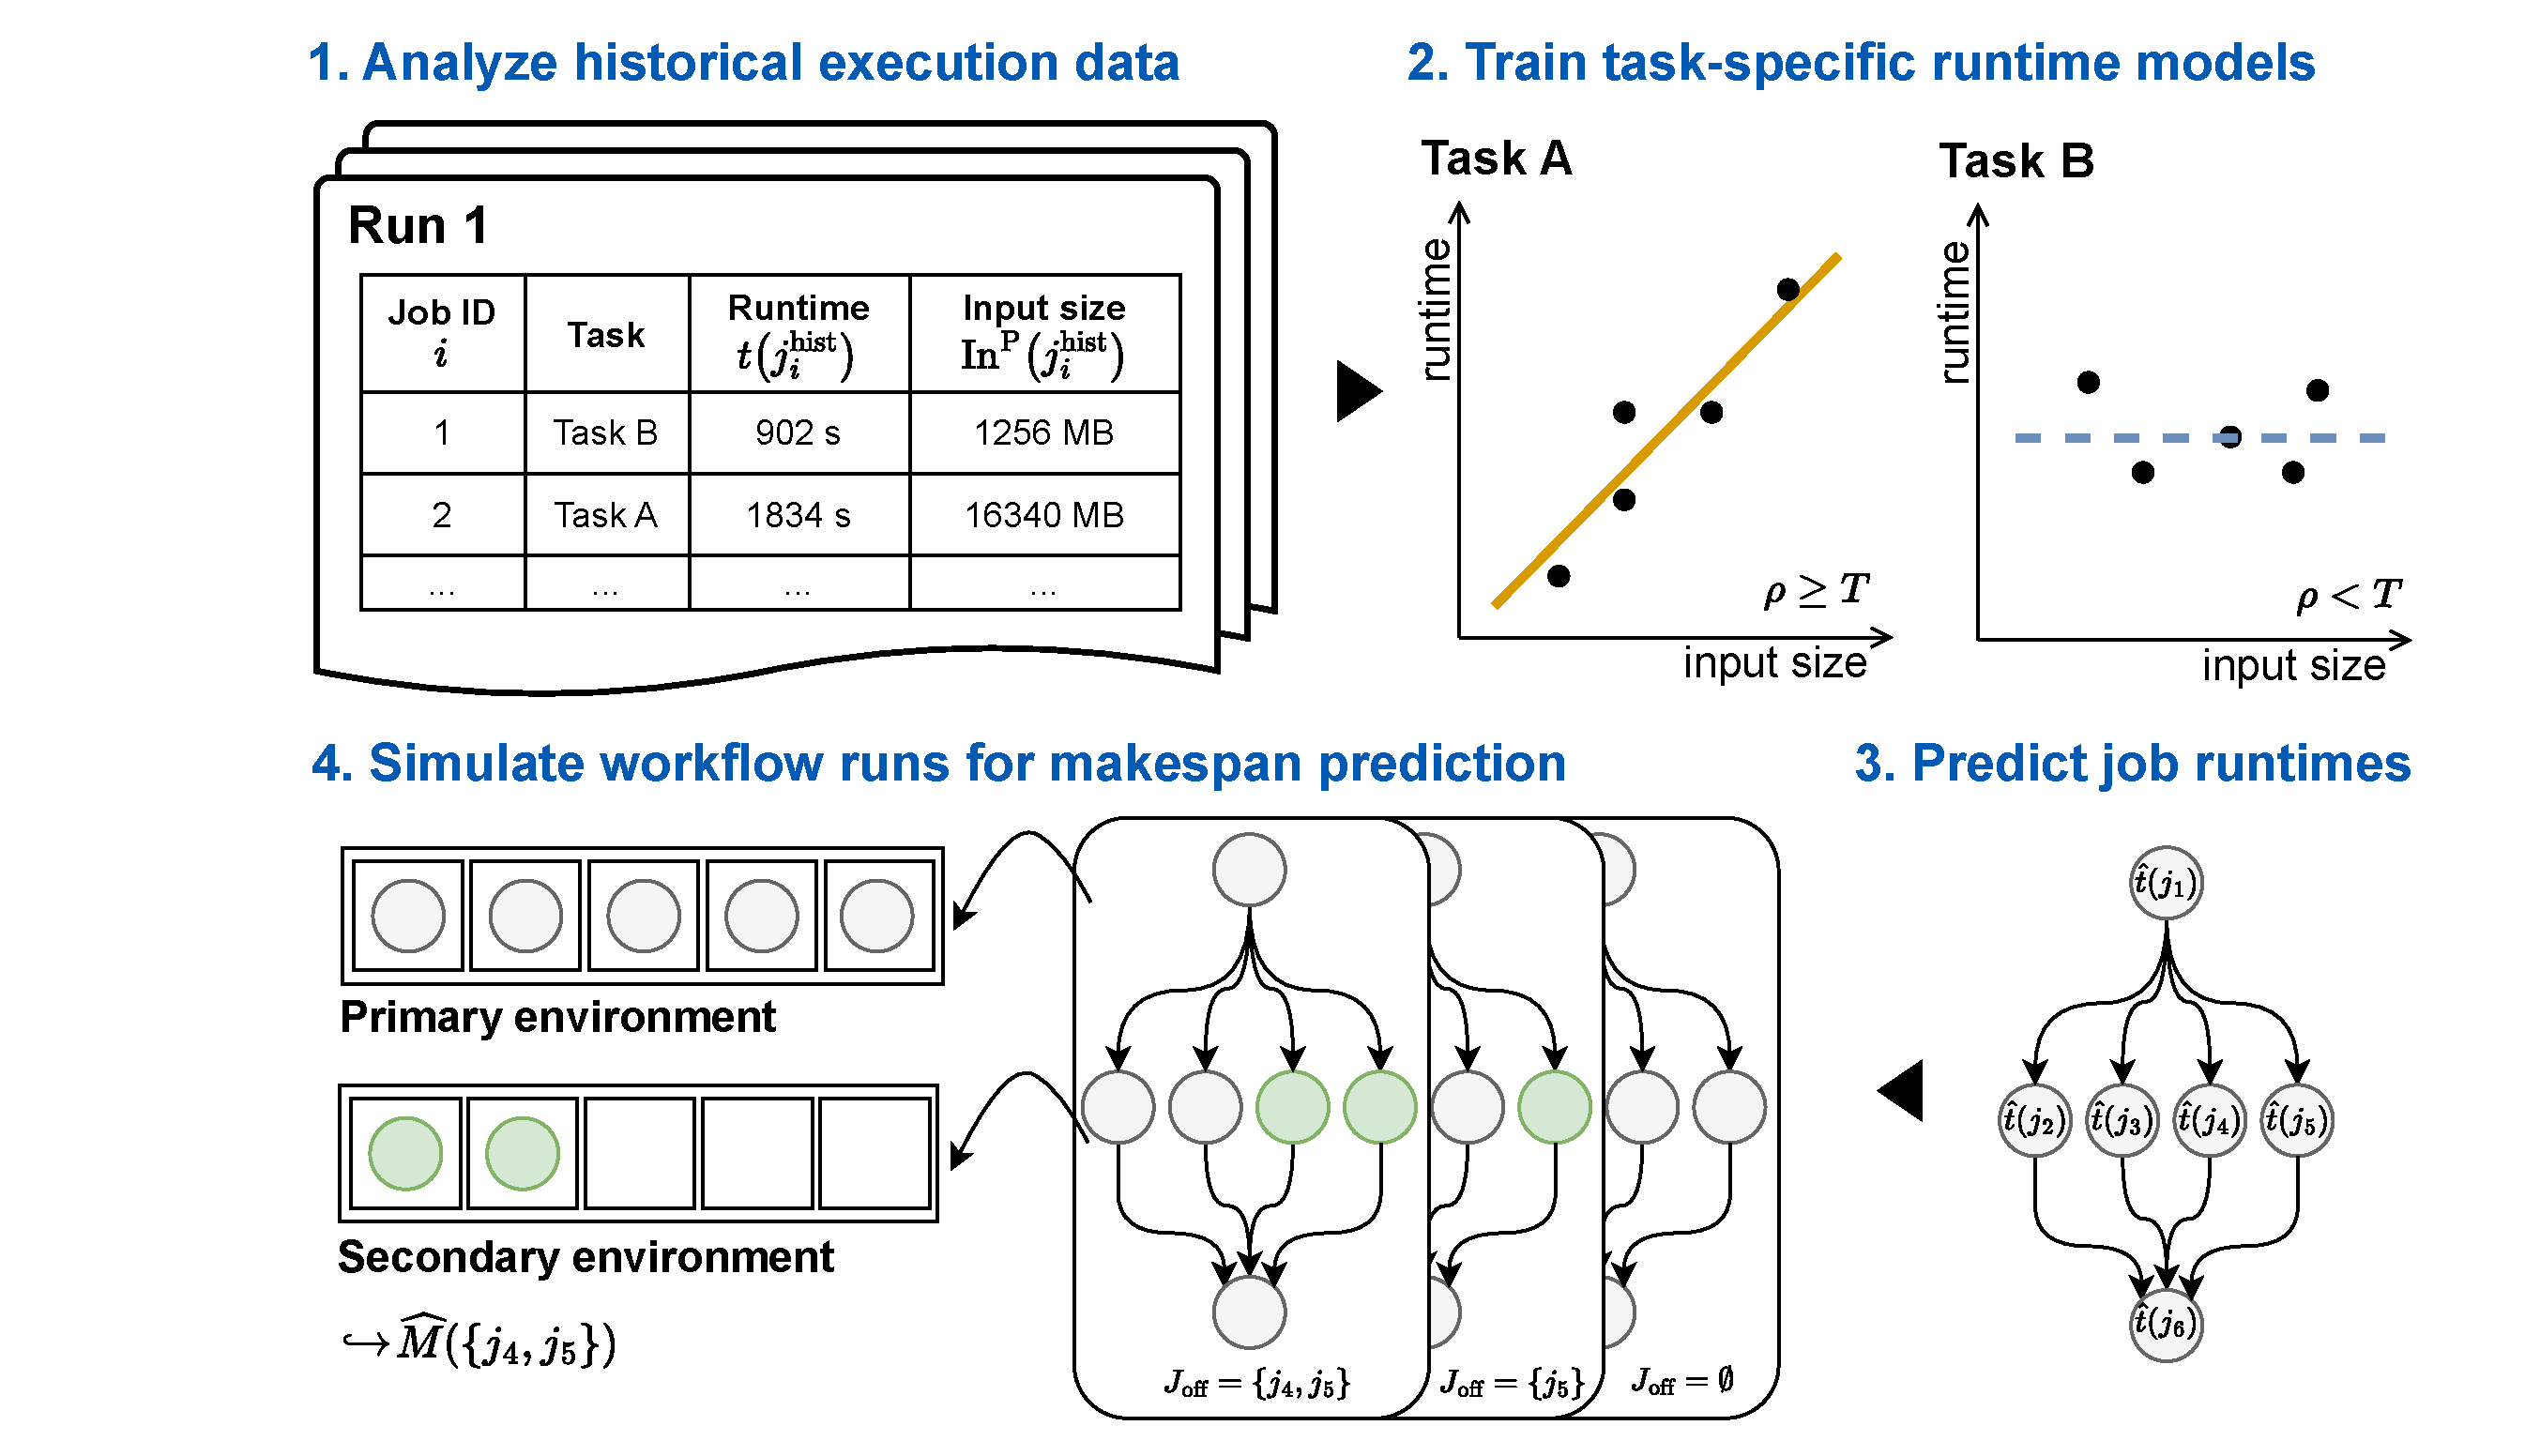
\includegraphics[width=0.8\linewidth]{./img/approach_overview.drawio.pdf} \caption{Overview of the multi-cluster makespan prediction approach} \label{fig:approach_overview} 
\end{figure*}

At a high level, our approach introduces makespan prediction to simulate job offloading under various selection criteria, thereby aiming at identifying offloading configurations that meet the user's requirement.
As a workflow is composed of a set of jobs $J$, its makespan is influenced by the runtimes $t(j)$ of these jobs $j \in J$, their dependencies, and the extent of job parallelization.
Since workflow makespan directly depends on job runtimes, we implement a two-step prediction approach:
We first predict the runtimes of all jobs in $J$ and then use these predictions to estimate the workflow makespan over the multi-cluster environment. 
Fig.~\ref{fig:approach_overview} illustrates the overview of the proposed multi-cluster prediction approach. Whereas phases 1 and 2 represent necessary pre-processing procedures, phases 3 and 4 together constitute the two-step predictive offloading framework.

\subsubsection{Phase 1}
In the first phase, we analyze the workflow execution, extracting all historical jobs $J^\text{hist} = \{j_1^\text{hist}, j_2^\text{hist}, \dots j_k^\text{hist}\}$, including their runtimes $t(j_i^\text{hist})$ and their primary input data sizes $\text{In}^\text{P}(j_i^\text{hist})$ (the sum over all input files). We also determine $\text{In}^\text{P-A}(j_i^\text{hist})$, defined as \[ \text{In}^\text{P-A}(j_i^\text{hist}) = \sum_{j \in \text{Anc}(j_i^\text{hist})} \text{In}^\text{P}(j) \] where $\text{Anc}(j_i^\text{hist})$ is the set of all ancestor jobs of $j_i^\text{hist}$. Determining $\text{Anc}(j_i^\text{hist})$ requires reconstructing the DAG of jobs for all workflow runs of the historical job records. In the following, we refer to the sum $\text{In}^\text{P}(j_i^\text{hist}) + \text{In}^\text{P-A}(j_i^\text{hist})$ as the \textit{combined primary input data size} of job $j_i^\text{hist}$.

\subsubsection{Phase 2}
 In the second phase, we train task-specific runtime models. 
 %The model training procedure takes inspiration from Bader et al. \cite{bader_lotaru_2024}, but relies on simple linear instead of Bayesian regression. 
 For each task, we consider all associated historical job records, independent of the workflow run. For a task with $k$ historical job records, this leaves us with a dataset $\mathcal{D}^\text{hist}$ of $k$ pairs of combined primary input data size and runtime: \[ \mathcal{D}^\text{hist}=\left\{\left(\text{In}^\text{P}(j_i^\text{hist}) + \text{In}^\text{P-A}(j_i^\text{hist}),\; t(j_i^\text{hist})\right)\right\}_{i=1}^{k}. \] 
 
 First, we check if a task's job runtimes scale linearly with their combined primary input data size. 
 %Bader et al. \cite{bader_lotaru_2024} demonstrated that runtime often correlates with input data size for bioinformatics tasks, but not for all such tasks. 
 In addition, even if a task's job runtimes correlate with input data size, they must not necessarily correlate with combined primary input data size.
 Accordingly, we compute the Pearson correlation coefficient $\rho$ for the data points in $\mathcal{D}^\text{hist}$. If $\rho \geq T$ for a threshold $T$, we assume linearity and train a linear regression model for that task with $\mathcal{D}^\text{hist}$ as training data. Then, for any job $j \in J$ derived from that task, the runtime prediction $\hat{t}(j)$ is given by: \[ \hat{t}(j) = \beta_{0} + \beta_{1} (\text{In}^\text{P}(j) + \text{In}^\text{P-A}(j)), \] where \( \beta_{0} \) and \( \beta_{1} \) are the task-specific regression coefficients. If $\rho < T$, the runtime prediction is instead defined as \[ \hat{t}(j) = \mathrm{median}\left\{ t\!\left(j_i^\text{hist}\right) \right\}_{i=1}^k. \]
 
\subsubsection{Phase 3 and 4}
In the third and fourth phase, we predict the runtimes $\hat{t}(j)$ of all jobs $j \in J$ and the resulting makespan of the workflow. To this end, we simulate workflow runs with varying $J_{\text{off}} \subseteq J$, predicting the particular makespan for each configuration. 

We intend to identify the optimal offloading configuration $J_{\text{off}}^*$ and its makespan prediction $\hat{M}(J_{\text{off}}^*)$. 
However, the naive approach of simulating all possible configurations $J_{\text{off}}$ is not feasible for large workflows, as the number of configurations grows exponentially with the number of jobs: There exist $|\mathcal{P}(J)|=2^{|J|}$ possible configurations $J_{\text{off}}$, where $\mathcal{P}(J)$ denotes the power set of $J$. Therefore, we propose a heuristic approach that iteratively selects jobs for offloading. The selection of jobs is based on an offloading strategy $\mathcal{S}$, which determines the order in which jobs are chosen and is discussed in detail in section \ref{par:makespan_prediction} and \ref{par:offloading-strategies}.


\subsection{Adaptive Multi-Cluster Offloading Heuristic}
\label{subsec:heuristic}
In this section, we provide a detailed description of how the results obtained in phase 3 (see Figure \ref{fig:approach_overview}) are utilized to perform makespan prediction in a multi-cluster environment (phase 4). Subsequently, these makespan predictions are then employed to determine the subset of jobs that should be offloaded.
The goal of our approach is that for a given $\mathcal{S}$, we compute the smallest set $J^{\mathcal{S}}_\text{off} \subseteq J$ such that $\hat{M}(J^{\mathcal{S}}_\text{off}) \leq D$. 
It is reasonable to assume that $J^{\mathcal{S}}_\text{off}$ is associated with the lowest cost out of all $J_{\text{off}} \subseteq J$ for $\mathcal{S}$ that meet the deadline, as the cost function strictly increases with the number of jobs (see Section~\ref{par:cost-estimation}). Finding $J_{\text{off}}^*$ is then equivalent to finding the offloading strategy $\mathcal{S}^*$ that minimizes $\hat{C}(J^{\mathcal{S}}_\text{off})$. This considerably reduces the search space, as only a subset of all possible offloading configurations is evaluated. At the same time, we might only find a local optimum, as the global optimum is not guaranteed to be within the search space.

% Prediction Aspect
\begin{algorithm}[h]
\label{lst:predict_workflow_makespan}
\caption{Workflow Makespan Prediction}
\SetKwInOut{Parameter}{Parameters}
\Parameter{\\
    \var{$D$} : Deadline (maximum makespan) \\
    \var{$\mathcal{S}$} : Offloading strategy \\
    }

\If{\var{$\mathcal{S}$} is deadline-aware}{
    \var{$J'_\text{off}$} $\gets$ $\emptyset$\;

    \var{$\hat{M}$}, \var{$J^{\mathcal{S}}_\text{off}$}, \var{$J_{\text{def}}$} $\gets$
    \func{simulateWorkflowRun}(\var{$\mathcal{S}$}, \var{$J'_\text{off}$})\;
    \While{\var{$\hat{M}$} $>$ \var{$D$}}{

        \If{\var{$J_{\text{def}}$} $\setminus$ \var{$J'_\text{off}$} $=$ $\emptyset$}{
            break\;
        }
        update \var{$J'_\text{off}$} by selecting job from \var{$J_{\text{def}}$} $\setminus$ \var{$J'_\text{off}$}\;
        \func{simulateWorkflowRun}(\var{$\mathcal{S}$}, \var{$J'_\text{off}$})\;
        update \var{$\hat{M}$} with \var{$\hat{M'}$} and \var{$J^{\mathcal{S}}_\text{off}$} with \var{$J'^{\mathcal{S}}_\text{off}$}\;
    }
}
\Else{
    \var{$\hat{M}$}, \var{$J^{\mathcal{S}}_\text{off}$}, \var{$J_{\text{def}}$} $\gets$
    \func{simulateWorkflowRun}(\var{$\mathcal{S}$}, None)\;
}

\Return \var{$\hat{M}$}, \var{$J^{\mathcal{S}}_\text{off}$}\;
\end{algorithm}
\paragraph{Multi-cluster Makespan Prediction under Offloading}\label{par:makespan_prediction}

The effective makespan $M(J_{\text{off}})$ and offloading cost $C(J_{\text{off}})$ of a workflow are only known after execution. Yet it is of great interest to find the optimal offloading configuration $J_{\text{off}}^*$ before execution, saving resources by avoiding expensive trial-and-error runs. 
Therefore we propose an approach to predict workflow makespan and associated offloading cost in advance.
We denote these predictions as $\hat{M}(J_{\text{off}})$ and $\hat{C}(J_{\text{off}})$. 

Algorithm~\ref{lst:predict_workflow_makespan} presents the heuristic more formally.
As parameters, it accepts a deadline $D$ and an offloading strategy $\mathcal{S}$.
It returns the predicted makespan $\hat{M}$, and the associated set of offloaded jobs $J^{\mathcal{S}}_\text{off}$. (For simplicity, we deviate slightly from the notation above, using $\hat{M}$ instead of $\hat{M}(J^{\mathcal{S}}_\text{off})$.) At different points, the algorithm calls the function \code{simulateWorkflowRun}. As input, this function accepts an offloading strategy and a set of jobs to be offloaded in the simulation and it returns $\hat{M'}$, $J'_\text{off}$ and $J_{\text{def}}$. 
%If the set is \code{None}, the offloaded jobs will be selected implicitly depending on the offloading strategy. %\code{simulateWorkflowRun} will be described in greater detail in Algorithm~\ref{lst:simulate_workflow_run}. It returns the predicted makespan $\hat{M'}$, the set of offloaded jobs $J'_\text{off}$ and the set of deferred jobs $J_{\text{def}}$. These are the jobs that had to be deferred at one point in the simulation, as they could not be executed immediately in one of the execution environments due to resource exhaustion.
The algorithm differentiates between deadline-aware strategies, which approach $D$ by iteratively simulating job selection until $D$ is met, and deadline-agnostic strategies, which do not consider any deadline (see Section~\ref{par:offloading-strategies} for details).
If $\mathcal{S}$ is deadline-agnostic (line 11), the algorithm simply calls the \code{simulateWorkflowRun} function once and returns the resulting makespan prediction and set of offloaded jobs.
If $\mathcal{S}$ is deadline-aware, the algorithm explicitly selects the jobs to be offloaded $J'_\text{off}$ and calls \code{simulateWorkflowRun} potentially many times.
With $\hat{M}'$, we denote the latest makespan prediction, and with $\hat{M}$, the best makespan prediction found so far.
Similarly, with $J'_\text{off}$, we denote the latest set of jobs selected for offloading, and with $J^{\mathcal{S}}_\text{off}$, the best set found so far, which is associated with $\hat{M}$.
In a first step, $J'_\text{off}$ is the empty set and the workflow is simulated once (lines 2-3).
If this results is a makespan prediction $\hat{M} \leq D$, the deadline can be met without offloading any jobs, and the algorithm returns.
Otherwise, the algorithm iteratively chooses additional jobs to be offloaded (lines 4-9).
In each iteration, as long as there is a job that has been deferred in the last simulation run and has not yet been offloaded (line 5), another job is added to $J'_\text{off}$ (line 7).
By restricting the selection to $J_{\text{def}} \setminus J'_\text{off}$, we ensure that only jobs that could not be executed in the primary environment are considered for offloading.
\begin{algorithm}[t]
\label{lst:simulate_workflow_run}
\caption{Workflow Run Simulation}
\SetKwInOut{Parameter}{Parameters}
\Parameter{\\
    \var{$\mathcal{S}$} : Offloading strategy \\
    \var{$J'_\text{off}$} : Set of jobs that must be offloaded
    }

\vspace{0.5em}

%Initialize \var{job\_queue}, \var{deferred\_jobs} as empty queues\;
%\vspace{0.2em}
%Initialize \var{time\_left\_per\_job} as empty map\;
%\vspace{0.2em}
Load \var{DAG}, \var{predictions}, \var{Q} and set \var{$\hat{M'}$} to 0\;
\vspace{0.5em}

\While{there are unfinished jobs in \var{DAG}}{
    \vspace{0.2em}
    add newly runnable \var{job} from \var{DAG} to \var{Q}\;
    %add newly runnable jobs $j \in \var{DAG}$ to \var{Q}\;
    \vspace{0.2em}
    \While{\var{Q} $\neq$ $\emptyset$}{
        \vspace{0.2em}
        %\var{job} $\gets$ \var{job\_queue}\func{.pop()}\;
        \vspace{0.2em}
        get \var{job} from \var{Q} and \func{assignJobToNode}(\var{job}, \var{$\mathcal{S}$}, \var{$J'_\text{off}$})\;
        %\var{node} $\gets$ \func{assignJobToNode}(\var{job}, \var{$\mathcal{S}$}, \var{$J'_\text{off}$})\;
        \vspace{0.2em}
        \If{\var{node} is found}{
            \vspace{0.2em}
           %\tcp{map job to runtime prediction}
            %\var{time\_left\_per\_job}[\var{job}] $\gets$ \var{predictions}[\var{job}]\; 
            \var{remaining\_job\_runtimes} $\gets$ runtime prediction \var{$\hat{t}$} for \var{job}\;
        }
        \vspace{0.2em}
        \Else{
            \vspace{0.2em}
            %\var{deferred\_jobs}\func{.push}(\var{job})\;
            store \var{job} and add to \var{Q} in next scheduling interval;
        }
    }
    %\vspace{0.2em}
    %\var{job\_queue}\func{.push}(\var{deferred\_jobs})\;
    %\vspace{0.2em}
    %\var{deferred\_jobs}\func{.clear()}\;
    %\vspace{0.2em}
    %\If{\var{time\_left\_per\_job} not empty}{
    \If{\var{remaining\_job\_runtimes} not empty}{
        \vspace{0.2em}
        %\var{time\_passed} $\gets$ min(\var{time\_left\_per\_job})\;
        \var{step\_time} $\gets$ min(\var{remaining\_job\_runtimes})\;
        update \var{$\hat{M'}$} by adding \var{step\_time}\;
        %\vspace{0.2em}
        %\var{$\hat{M'}$} $\gets$ \var{$\hat{M'}$} + \var{time\_passed}\;
        %\vspace{0.2em}
        %\var{newly\_finished\_job} $\gets$ argmin(\var{time\_left\_per\_job})\;
        %\vspace{0.2em}
        %\var{time\_left\_per\_job}.remove(\var{newly\_finished\_job})\;
        %\vspace{0.2em}
        \ForEach{\var{job} in \var{remaining\_job\_runtimes}}{
            \vspace{0.2em}
            %\var{time\_left\_per\_job}[\var{job}] $\gets$ \var{time\_left\_per\_job}[\var{job}] - \var{time\_passed}\;
            update each \var{job} by \var{step\_time}\;
        }
        \vspace{0.2em}
        reset resources of \var{node} that ran the latest \var{job} and remove from \var{DAG}\;
        %\vspace{0.2em}
        %mark \var{newly\_finished\_job} in \var{DAG} as finished\;
    }
}
\vspace{0.2em}
\Return \var{$\hat{M'}$}, all offloaded jobs, all jobs deferred at least once\;
\end{algorithm}
A job could be deferred even when offloaded if the secondary execution environment has insufficient resources. This case is most relevant for scenarios where the secondary environment is not a cloud environment with virtually unlimited resources, but another cluster.
The selection of the next offloaded job is based on $\mathcal{S}$.
Then, \code{simulateWorkflowRun} is called again with the updated set of offloaded jobs (line 8).
If the resulting makespan prediction $\hat{M}'$ is the best one found so far, $\hat{M}$ and $J^{\mathcal{S}}_\text{off}$ are updated (line 9).

If the secondary environment has insufficient resources, adding jobs to $J'_\text{off}$ does not necessarily lead to a smaller makespan prediction, as jobs could be deferred again.
In case there are no more deferred jobs that have not yet been offloaded, the algorithm aborts and returns the current $\hat{M}$ and $J^{\mathcal{S}}_\text{off}$ (lines 11-12).
This is because we assume that jobs should only be offloaded if they cannot be run in the primary execution environment due to resource exhaustion.
Given assumption A1 (Section~\ref{sec:problem}), we conclude that jobs running in the secondary environment would not finish earlier than in the primary environment, and therefore offloading them would not reduce the makespan but instead only increase the cost.
Although in that case the deadline cannot be met (line 6), $J^{\mathcal{S}}_\text{off}$ can still be considered the best-effort offload configuration.


% Simulation Aspect 
\paragraph{Simulation-based Offloading Optimization}
\begin{table}[t] 
\caption{Offloading strategies and their selection criteria} 
\centering 
\footnotesize 
\begin{tabular}{l|l} 
\textbf{Strategy} & \textbf{Description} \\ \hline  (1) PEFO & Offloads jobs when no primary resources are available  \\ (2) LJF & Offloads jobs with largest predicted runtime $\hat{t}(j)$ \\ (3) SISF & Offloads jobs with smallest primary input size $\text{In}^\text{P}(j_i^\text{hist})$
\end{tabular} 
\label{tab:offloading-strategies} 
\end{table} 
Given the above considerations, Algorithm~\ref{lst:simulate_workflow_run} represents the \code{simulateWorkflowRun} function invoked in Algorithm~\ref{lst:predict_workflow_makespan}.
As parameters, it accepts the offloading strategy $\mathcal{S}$ and the set of jobs to be offloaded $J'_\text{off}$.
The scheduling queue \code{Q} is processed until all jobs have been assigned to a node (line 5) or have been deferred because no node had sufficient resources (line 9).
The \code{assignToNode} function maintains an internal representation of simulated, available resources for each node in both cluster environments. If no node can provide sufficient resources, the function returns \code{None}, and the job is deferred.
The data structure \code{remaining\_job\_runtimes} serves to track the remaining runtime of running jobs, which at first is their runtime prediction (line 7).
Additionally it is ensured that, for deadline-aware strategies, a job is offloaded if and only if it belongs to $J'_\text{off}$, since the offloaded jobs have already been selected according to strategy $\mathcal{S}$. In the case deadline-unaware offloading, a job is only offloaded when the primary environment cannot meet its resource requirements at scheduling time and every job is assigned to the primary environment.
Once \code{Q} has been processed, deferred jobs are moved back into the queue to be retried in the next scheduling iteration. After each iteration, if there are running jobs, the job with the smallest remaining runtime is marked as finished. Its remaining runtime is added to the makespan and subtracted from the remaining runtimes of all other running jobs (lines 11-14), and the resources it used are released (line 15). In the next iteration, all jobs that become runnable due to this completion are added to \code{Q} and the loop continues until \code{Q} = $\emptyset$.

\paragraph{Offloading Strategies}\label{par:offloading-strategies}

Table \ref{tab:offloading-strategies} specifies the job selection criteria for offloading to a secondary environment. By comparing the results of Algorithm~\ref{lst:predict_workflow_makespan} between strategies, we select the strategy $\mathcal{S^*}$ with minimal offload cost $\hat{C}(J^{\mathcal{S^*}}_{\text{off}})=\hat{C}(J^{*}_{\text{off}})$. We consider both deadline-aware and deadline-agnostic strategies.

\begin{enumerate}

    \item \textbf{Primary Environment Fully Occupied (PEFO)} offloads a job exclusively when the primary environment does not possess sufficient resources to enable its immediate execution. PEFO serves as an offloading baseline, where the primary environment is constrained in capacity but otherwise unencumbered, whereas the secondary environment is associated with higher operational costs.
    \item \textbf{Longest Job First (LJF)} selects the job for offloading with the longest predicted runtime and is suited to settings where offloading incurs an additional overhead such as data transfer times or network latency, as long-running jobs are more likely to amortize such overhead. 
    \item \textbf{Smallest Input Size First (SISF)} selects jobs with the smallest combined primary input data size $\text{In}^\text{P}(j_i^\text{hist})$ and targets cases where offloading cost scales with input size. 
\end{enumerate}

To this end, these strategies are considered appropriate for the given configuration of task attributes, while additional selection criteria can be defined to account for specific job types or information regarding resource availability.

\paragraph{Workflow Cost Estimation}\label{par:cost-estimation}
% Makespan prediction yields For a given offloading configuration $J^{\mathcal{S}}_{\text{off}}$, we can predict the associated cost using the runtime predictions $\hat{t}(j_i)$ for $j_i \in J_{\text{off}}$.
For a given offloading configuration $J_{\text{off}}$, we model the cost prediction function $\hat{C}(J_{\text{off}})$ as a linear combination of job-level resource usages, weighted by unit cost factors:
\[
\hat{C}(J_{\text{off}}) = \sum_{j \in J_{\text{off}}} \hat{t}(j) \cdot \big(
\alpha_{\text{cpu}} \cdot \text{cpu}(j) +
\alpha_{\text{mem}} \cdot \text{mem}(j) +
\alpha_{\text{stor}} \cdot \text{stor}(j)
\big)
\]

Here, \(\hat{t}(j) \in \mathbb{R}_{\geq 0}\) denotes the predicted runtime of job \(j\) in hours, while \(\mathrm{cpu}(j)\), \(\mathrm{mem}(j)\), and \(\mathrm{stor}(j)\) denote the requested number of vCPUs, memory in GiB, and ephemeral storage in GiB, respectively. The coefficient \(\alpha\) corresponds to the unit price per resource in Table \ref{tab:unit-cost-factors}.

The values of these unit prices are based on the pricing of AWS Fargate (eu-central-1 region, Linux/X86 platform) as of 22 July 2025\footnote{\url{https://aws.amazon.com/fargate/pricing}}.
If jobs do not specify resource requests, we assume a default request of 1~vCPU, 2~GiB of memory and 20~GiB of ephemeral storage.

Thus, for any $J^{\mathcal{S}}_\text{off}$ found by Algorithm~\ref{lst:predict_workflow_makespan}, we can compute the associated cost prediction $\hat{C}(J^{\mathcal{S}}_\text{off})$ using the runtime predictions $\hat{t}(j)$ calculated earlier and the resource requests of each job.
In case a workflow definition does not specify resource requests for a job, we can fall back to default values (e.g., 1 vCPU, 2 GiB memory, 20 GiB storage).
%Note that the cost function does not model possible ingress or egress costs for transferring data to or from the secondary execution environment, which might be incurred by offerings of public cloud providers.

\begin{table}[t]
\caption{Unit cost factors used in the cost model}
\centering
\footnotesize
\setlength{\tabcolsep}{4pt}
\begin{tabular}{l|c|l}
\textbf{Resource} & \textbf{Unit Cost (\$)} & \textbf{Billing Basis} \\
\hline
CPU     & 0.04656  & per vCPU-hour \\
Memory  & 0.00511  & per GiB-hour \\
Storage & 0.000132 & per GiB-hour (ephemeral)
\end{tabular}
\label{tab:unit-cost-factors}
\end{table}


